\documentclass[utf8]{article}




%% Language and font encodings
\usepackage[english]{babel}
%\usepackage[utf8]{inputenc}
\usepackage[T1]{fontenc}

%% Sets page size and margins
%\usepackage[a4paper, top=3cm,bottom=2cm,left=3cm,right=3cm,marginparwidth=4cm]{geometry}
\usepackage[papersize={10in, 12in}, top=3cm,bottom=2cm,left=2in,right=2in,marginparwidth=1.8in]{geometry}


%% Title style
\usepackage{stringstrings}
\usepackage[explicit]{titlesec}
\usepackage{sectsty}
%\usepackage{titlesec}

%\sectionfont{\capitalize}



%\newcommand\SentenceCase[1]{%
%	\caselower[e]{#1}%
%	\capitalize[q]{\thestring}%
%}
%\titleformat{\section}{\normalfont\Large\bfseries}{\thesection}{1em}{\SentenceCase{#1}\thestring}




%% Useful packages
\usepackage[dvipsnames,table,xcdraw]{xcolor}
\usepackage[round]{natbib}
\usepackage{amsmath}
\usepackage{graphicx}
\usepackage[colorlinks=true, allcolors=blue]{hyperref}
\usepackage{authblk}
\usepackage{float}
\usepackage{tikz}




%% acronym
\usepackage{acronym}
\newacro{ntic}{non-trivial informational closure}
\newacro{ic}{informational closure}
\newacro{cg}{coarse-grain}
\newacro{cging}{coarse-graining}
\newacro{cged}{coarse-grained}
\newacro{ncg}{neural coarse-graining}



% =================================== Macro ================================== %
\usepackage[colorinlistoftodos]{todonotes}
\usepackage[at]{easylist}
\usepackage{tcolorbox}


% Meaning of colours --------------------------------------------------------- %
%	Red: Important and Critical
%	Orange: Todo
%	Blue: Topic and Guideline
%	Purple: Murmur, talking to myself
%	Green: Question, Call for help, Open for opinions and comments
%	Brown: Need Wording 
% ---------------------------------------------------------------------------- %


% Real content
	% Finished part
	% Outline items that can be integrated into main text
		\newenvironment{ants}
			{
			 \begin{easylist}[itemize]
			}
			{
			\end{easylist}
			}
% Funcitonal content
	% Quotes
		\newcommand{\rewrite}[1]{\textcolor{ForestGreen}{\textit{"#1"}}\newline}
		
	% todo
		% figure

		\newcommand{\includegraphicsTodo}[2][]{%
			\tcbox[%
				adjusted title=\LARGE To Be Modified,
				halign title=right,
				colbacktitle=Orange!75!White,
				coltitle=Black,
				colframe=Red!60!White,
				boxrule=1mm,
				colback=white%
				]{\includegraphics[#1]{#2}}}		
		
	
	% Highlight
		\newcommand{\highlight}[2][Yellow]{\colorbox{#2}}
	
		% Highlight and comment
		\newcommand{\highlightAndComment}[3][Yellow]{\todo[color=#1]{#3}\colorbox{#1}{#2}}
	
	% rewording
		\newcommand{\rewording}[1]{\textcolor{RawSienna}{[[ REWORDING | #1 ]]}}
		
	% Need reference 
		\newcommand{\needref}[1]{%
			\ifthenelse{\equal{#1}{}}{%
				\todo[color=White, linecolor=BlueViolet]{\textcolor{BlueViolet}{Ref}}}{%
				\todo[color=White, linecolor=BlueViolet]{\textcolor{BlueViolet}{Ref: #1}}%
				}%
		}

	% idea
		% text idea
			\newcommand{\idea}[1]{\noindent
				\textcolor{Plum}{[[ #1 ]]}}	
		
		% box idea
			\newcommand{\ideaBox}[1]{
				\begin{tcolorbox}[hyphenationfix, width=12cm, colback=Thistle!50!white, flush right]
					#1
				\end{tcolorbox}
			}
		
		% callout idea
			\newcommand{\ideaCallout}[1]{\todo[color=Thistle, size=\small]{#1}}
		
	% guildline and direction
		\newcommand{\toWrite}[1]{\noindent
			\textcolor{Cyan}{\textbf{[[ #1 ]]}}}
		
	% call for help
		\newcommand{\callforhelp}[1]{\todo[color=SpringGreen]{#1}}
		\newcommand{\martin}[1]{\todo[color=SpringGreen]{@Martin:\\#1}}
		





% ============================================================================ %
%                                     Title                                    %
% ============================================================================ %
\title{A neural coarse graining theory of consciousness}



% ============================================================================ %
%                                    Authors                                   %
% ============================================================================ %
\author[1]{Acer Y.C. Chang\thanks{acercyc@araya.org}}
\author[1]{Martin Biehl\thanks{martin@araya.org}}
\author[1]{Ryota Kanai\thanks{kanair@araya.org }}
\affil[1]{ARAYA, Inc., Tokyo, Japan}


\begin{document}
	\maketitle
	\tableofcontents


	\begin{abstract}
		Neural systems process information through different levels of organisation in a hierarchical manner. Information at lower levels is finer-grained and can be coarse-grained for higher level computation. However, one is aware of information processed only at specific levels. Theorists have addressed this issue. For example, the intermediate level theory of consciousness suggests that the intermediate level seems to be privileged with respect to consciousness. It is true that we do not experience information processed by individual neurons which is always highly noisy. Besides, we have no conscious experience from interpersonal activities albeit massive interactions among individuals. Instead, neurophysiological evidence has been showing that conscious experience tends to covary with information encoded in coarse-grained neural states such as neural population codes. We argue that the neural states within the scope of the informational closure determine the contents of consciousness and brain processes outside apart from the representations of that level remain unconscious. This argument suggests a distinction between conscious and unconscious processing and provides a generic computational framework. Finally, using the deep learning network, we can measure informational closure in deep hidden layers. Our preliminary results show that informational closure representation emerged after learning. We further decoded the information from the representation and compared it with human conscious perception.
	\end{abstract}
	
	
	\section*{Keywords:} 
	Keywords: theory of Consciousness, informational closure, neural coarse-graining, level of analysis
	
	% ============================================================================ %
	%                                     Start                                    %
	% ============================================================================ %
	
	
	\section{Introduction}
	
		\begin{ants}
			
			%% Story about a cell
				@ Imagining you are a neuron in Bill's brain. Your daily work is to collect neurotransmitters through dendrites from other neurons, accumulate membrane potential, and finally send signals to other neurons through action potentials. 
				
				@ You have no idea that you are one of neurons in Bill's supplementary motor area and is now involved in motor control processing while Bill is reaching his hand to grab a cup. 
				
				@ You are totally ignorant of the intension, the goal, and the motor plan that Bill is having now even thought you are part of the physiological substrate responsible for this action. 
				
				@ The same story also happens to Bill's conscious mind. In his conscious experience, he is unaware of everything you do and even not able to know your existence if Bill never studies neuroscience.
				
				@ It seems that information you are processing and information shows in Bill's conscious percept are divorced from each other. 
				
				@ \idea{Need a ending sentence here}
				
				@ ====================================
				
				
													
				% @ Strikingly, not only you are ignorance of Bill's intention but also Bill has no conscious awareness of your behaviour. If your work contributes some part of Bill's conscious perception or intention to act. 
			
			
			%% scale
				
				@ It seems to be true that we are unable to consciously access information processed at every scale in the neural system. Only information at certain levels of coarse-graining is able to be parts of conscious contents. 
				
				@ When we focus on microscopic level of neural systems, information processing in individual neurons is highly noisy and state transitions of neurons are highly stochastic \citep{Goldwyn2011, White2000}. However, instead of stochastic action potentials and fluctuation of random noise at microscopic levels, what we are aware of in our conscious contents shows astonishing stability and high robustness against to ubiquitous noise in the neural system \citep{mathis1995computational}.
				
				
				% Neurons fires all the time. However, those massive action potentials do not appear in our  conscious contents. 
			
				@ Likewise, at the macroscopic level, conscious experience does not associate with joint states of the full neural system because we have known that some parts of the neural system process information unconsciously (cerebellum for example \citep{lemon2010life}). 				
			
				@ Meanwhile, we don't experience "super-consciousness" when we have massive inter-individual interactions with other human-beings. Even though evidence has shown several types of collective information processing at human social groups levels \needref{collective intelligent in human, collective memory, collective behavioural, etc.}, those processes seem to depart from our individual conscious contents.
				
				
				@ \idea{Need a ending sentence here}

				@ ====================================				

			
			%% our argument
				@ In this article, we propose that consciousness \highlightAndComment[YellowGreen]{correlates}{Is this proper?} information processing at a certain coarse-grained level where the neural system creates a high degree of non-trivial informational closure. We further predict that \textit{levels} of consciousness are determined by the levels of informational closure and \textit{contents} of consciousness are determined by the concurrent states of the informational closure \citep{laureys2005neural, overgaard2010neural}.\todo{There must be a better way to reword this part}

				
				
			%% About this paper
				@ In the following sections, we first introduce non-trivial informational closure and its importance to information processing for human scale agents. 
				
				@ We argue that through coarse-graining the human neural system can achieves non-trivial informational closure at a specific coarse-grained level.
				
				@ We then propose that the state of the informational closure correlates the state of consciousness for both levels and contents which can be explained and computationally quantified and predicted in this theory. 
				
				@ We discuss how this theory can concisely explain empirical results from previous studies and reconcile several current major theories of consciousness. 
				
				@ We finally provide predictions and testable approaches for this theory.
			
				
		\end{ants}

	
	
%		==================================================
%		\begin{ants}
%			
%			@ consciousness is information
%			
%			@ conscious contents
%				@@ \toWrite{lower level}
%				@@ Information processing of individual neurons are noisy.
%				@@ We don't have conscious content changes when individual neurons fire action potentials. 				
%				@@ Don't even mention ion channel dynamic. 
%				
%				
%				@@ \toWrite{Higher-level dynamic}
%
%				
%				
%				
%				
%			
%			@ For human, physics at our body scale are nearly follow classic physics, which is deterministic. 
%			
%			
%			@ \toWrite{Human tendency for active prediction }
%				@@ \cite{Stahl2015} \rewrite{
%					Given the overwhelming quantity of information available from the environment, how do young learners know what to learn about and what to ignore? We found that 11-month-old infants (N = 110) used violations of prior expectations as special opportunities for learning. The infants were shown events that violated expectations about object behavior or events that were nearly identical but did not violate expectations. The sight of an object that violated expectations enhanced learning and promoted information-seeking behaviors; specifically, infants learned more effectively about objects that committed violations, explored those objects more, and engaged in hypothesis-testing behaviors that reflected the particular kind of violation seen. Thus, early in life, expectancy violations offer a wedge into the problem of what to learn.}
%			
%			@ Intuitive physics \needref{Intuitive physics}
%			
%			@ However, sensory signal are always noisy. 			
%			
%			
%			@ We propose that consciousness is not related to particular neural architectures or location of the neural system.
%			
%
%		\end{ants}
	
	
	
	
	
	

	\section{Non-trivial informational closure\martin{todo}}
	
		\subsection*{Meaning of informational closure}
			\begin{ants}
				@ \rewrite{
					The notion of closure plays a prominent role in systems theory where it is used to identify or define the system in distinction from its environment} \cite{BERTSCHINGER.2006}
		
				@ \rewrite{
					Our theoretical interest concerns the type of system that is a unity for and by itself and not only for an external observer distinguishing some entity from the rest of the world. This requires a system that can be described as a whole without reference to its environment. In systems theory, this property is usually referred to as closure.}\citep{BERTSCHINGER.2006}
				
				@ \rewrite{
					These concepts of closure play an important role in the architecture of systems
					theory, because they are used to
					1. define the system (in distinction to its environment) and to 
					2. explain the autonomy of the system.}\citep{BERTSCHINGER.2006}
				
				@ \rewrite{
					Informational closure: The higher process is informationally closed, i.e., there is no information flow from the lower to the higher level. Knowledge of the microstate will not improve predictions of the macrostate.} \citep[p. 4]{PFANTE.2014}
				
								
			\end{ants}
	
	
		\subsection*{Definition of informational closure}
		
			\begin{figure}
				\includegraphicsTodo[width=\textwidth]{WritingMaterials/PDFXCview_2018-06-07_17-45-59.png} 
				\cite{BERTSCHINGER.2006} I need something like this 
				\caption{xxxx}
				\label{fig:AgentAndEnv}			
			\end{figure}

			
			\begin{ants}				
				@ Formally, then, a system is informationally closed if (almost) no information flows into it from the environment.
				
				@ \rewrite{
					The notion of informational closure refers to a situation where the information flow between the environment and the system tends to zero.} \cite{BERTSCHINGER.2006}
				
				@ Mathematically, informational closure can be define and measured by as the degree of information flowing from the environment to a system.
				\begin{equation}\label{eq:InformationFlow}
				\left.\begin{array}
				{rl}{J_{n}(E \rightarrow S )} & { = MI(S_{n+1};E_{n}|S_{n})} \\
				{ } & { = H(S_{n+1}|S_{n})-H(S_{n+1}|S_{n},E_{n})} \\
				{ } & { = H(E_{n}|S_{n})-H(E_{n}|S_{n},S_{n+1})} \\
				{ } & { = H(E_{n}|S_{n})-H(E_{n}|S_{n},S_{n+1})}
				\end{array}\right.
				\end{equation}
				
				
				@ \ref{eq:InformationFlow} can be rewritten as 
				\begin{equation}
				MI(S_{n+1};E_{n}|S_{n}) = 
				MI(S_{n+1};E_{n}) - (MI(S_{n+1};S_{n})-MI(S_{n+1};S_{n}|E_{n}))
				\end{equation}
				
			\end{ants}
		
		
		
		\subsection*{trivial case}
			\begin{ants}
				@ However, informational closure could be trivial.
				
				@ Information closure could be trivial. That is, when a system is fully independent from the environment, no information can flow into the system from the environment and also leak to the environment from the system. Equa. xxxx shows the mathematical description of trivial informational closure. When mutual information between the environment and system future state close to 0, and the system transition is independent from the environment, the system can reach informational closure. However, such systems do not have any functional meaning and evolutional advantages.
	
				@ \rewrite{
					A system that is independent from its environment trivially achieves informational closure.}  \cite{BERTSCHINGER.2006}
					\begin{equation}
						\left.\begin{array}
						{l}{MI(S_{n+1};E_{n})=0}\\
						{MI(S_{n+1};S_{n})-MI(S_{n+1};S_{n}|E_{n})=0}
						\end{array}\right.
					\end{equation}
			\end{ants}
		
		
		
		\subsection*{Non-trivial informational closure}
			\begin{ants}
				
				@ \citep{BERTSCHINGER.2006}
				@ \citep{guttenberg2016neural}

				@ \rewrite{The “informational closure” becomes non-trivial if the state contains information about the environment, i.e. $MI(S_{n+1};E_{n})\neq0$}
	
				@ We can define non-trivial informational closure (NTIC)
				
				@ Definition:\callforhelp{Which def is better? }
				
					@@
					\begin{equation}
					N T I C = H ( Y _ { t + 1} ) - H ( Y _ { t + 1} | Y _ { t } )
					\end{equation}
					\citep{guttenberg2016neural}
					
					@@
					\begin{equation}
					\left.\begin{array}{l}{ N T I C  : = M I ( S _ { n + 1} ; E _ { n } ,\dots ,E _ { n - m } ) - M I ( S _ { n + 1} ; E _ { n } ,\dots ,E _ { n - m } | S _ { n } ) }\\{  = M I ( S _ { n + 1} ; E _ { n } ,\dots ,E _ { n - m } ) - M I ( S _ { n + 1} ; E _ { n } | S _ { n } ) }\end{array} \right.
					\end{equation}
					\cite{BERTSCHINGER.2006}
					
					
				@ \rewrite{Modeling: The system reaches synchronization and internalizes the correlations observed in the environment by building up own structures.}
				
			\end{ants}
		

		
		\subsection*{Achieve non-trivial informational closure}
			\begin{ants}

				@ Accurately model deterministic environment 
				@ \rewrite{
					This demonstrates that a system exhibiting certain internal regularities as measured by $A^* = MI(Sn+1; Sn)$ can achieve informational closure either by gaining information about the environment or by increased autonomy, i.e. by becoming unpredictable or uncontrollable from the (13) environment. Therefore, information about the environment, i.e. modeling, and autonomy can be considered as complementary strategies for achieving informational closure.}
				
				@ By Action 
				
				@ In the next section, we claim that the neural system achieve NTIC through coarse-graining.
				
			\end{ants}


		
		\subsection*{informational closure and level identification \ideaCallout{maybe not necessary}}
		
		
		\subsection*{Biological Creature may try to achieve closure even the environment is not \ideaCallout{Maybe not necessary}}






	\section{Neural coarse-graining}
	
	
		\begin{ants}									
			
		
			%% About coarse-graining
%			@ \rewrite{
%				Coarse-graining: a method of reducing the complexity of a system by treating groups of atoms/molecules as single quasi-particles CG: coarse-grained}
%			
%			
%			@ \rewrite{
%				a number of different microstates,First, typically a number of different microstates, will realize the same value of the macro-variables of upper level causal theories.}
%			
%			
%			@ One consequence of coarse-graining is that it makes it permissible to ignore certain causal factors that would be relevant at more fine-grained level of description. \cite{price2007causation}
			
			
			
			%% Our argument
			@ We argues that the human neural system to achieve NTIC at a certain level of coarse-graining. 
			
			
			
			
			
			
			
			%% Macroscale Deterministic
			@ The environment that human scale agents interact with is approximately govern by Newton's law and therefore the state transitions \highlightAndComment{at a show time scale}{is this necessary?} are nearly deterministic.\callforhelp{Is there any good ref I can cite?} 
			
			@ \idea{Need something here}
			
			
			%% Noise
			@ However, information processing at the microscopic levels in the neural system is noisy. 
			
			
			@ \rewrite{
				neurons are noisy: the same pattern of activity never occurs twice, even when the same stimulus is presented.}
			
			
			%% Partial observable 
			@ And every individual sensor only receives a little amount of information about the environment. 
			
			@ Therefore, the dynamic of microscopic level is highly stochastic 
			
			
			%% coarse-graining is necessary
			@ Hence, to coarse-grain states of microscopic levels is necessary to represent and model the human-scale environment state and dynamics. 
			
			@ Coarse-graining is necessary to resist noise
			
			@ \rewrite{ The population will therefore be relatively insensitive to the loss of
				cells or noise in a small number of cells} \cite{eurich2000multidimensional}
						
			
			%% About consicousness
			@ More importantly, the information processing related to consciousness should not be situated at this level. Otherwise our conscious percept should be very noisy and unstable.
								
			
		\end{ants}
	
	
		\subsection{Coarse-graining in neural system}
			\begin{ants}
				
				@ We have known that the neural system uses various coding strategies to encode information at coarse-grained levels. 
				
				@ \toWrite{For examples}
				 
				 
				 
				%% temporal 
				@ temporal coarse-graining

					@@ firing rate coding
					
				
				

				@ Population coding
				
					@@ review ref
					
						@@@ \cite{Stanley2013}		
					
						@@@ \cite{QuianQuiroga2009}
				
					@@ Population coding is the idea that nervous systems signal and compute parameters using large populations of imprecise neurons, rather than one or a few precise neurons. 
	
					@@ \rewrite{
						As single neurons are not very informative, to obtain accurate information about sensory or motor variables some sort of population averaging must be performed.}
					
					
					@@ \rewrite{
						Neural population code: the set of response features of a population of neurons that carry all information about the considered stimuli. These features consist of spatio-temporal sequences of action potentials distributed across neurons and/or time.}
					
					@@ The diverse response selectivity of sensory neurons
					
					@@ \rewrite{
						How a neural population represents information is partly determined by the diverse selectivity of individual neurons \cite{Shamir2014}}
					
					@@ \rewrite{
						Population code (also ensemble code) denotes a code by which neural information is encoded in the spatiotemporal activity patterns of many neurons.
					} \cite{binder2009encyclopedia}		
				
				
				@ sensory hierarchy		
					@@ sensory hierarchy also shows characteristic of coarse-graining
					
					
					@@ Due to partial information that sensors can receive 
					
					@@ To form complex representation like shape, objects, coarse-graining is necessary. 
					
				
					@@ Through coarse-graining, \highlightAndComment{higher level}{might be confusing, need to think about the terminology here} cortical areas can integrate those partial information to infer hidden causes. 					
				
			\end{ants}		
		
		
		
			
		\subsection{\martin{todo}Neural coarse-graining}
			\begin{figure}
				\includegraphicsTodo[width=0.8\textwidth]{WritingMaterials/PDFXCview_2018-06-08_14-24-03.png}
				\caption{NCG \idea{I need to simplify this figure}\citep{guttenberg2016neural}}
				\label{fig:NCG}				
			\end{figure}
			
		
		
			\begin{ants}
				@ \citep{guttenberg2016neural} proposed an architecture, called neural coarse-graining (NCG), which aims to captures the emergent large-scale dynamics in the environment. 
				
				@ Achieving NTIC is the key objective to to extract out latent control parameters in the environment.
				
				@ During training, the objective of the architecture is to XXXXX\martin{todo}
				
				 
				@ \rewrite{
					The transform can learn to discard uninformative and unpredictable components of the signal in favor of the features which are both highly predictive and highly predictable.}\citep{guttenberg2016neural}
							
				
				
				@ \rewrite{
					The result is a semi-supervised algorithm which is capable of extracting latent parameters, segmenting sections of time-series with differing statistics, and building a higher-level representation of the underlying dynamics from unlabeled data}\citep{guttenberg2016neural}
				
			\end{ants}
		
		
		
			
		\subsection{The advantage of NCG}
			\subsubsection{Resistant to noise}
			\subsubsection{Predictive power}
			\subsubsection{Agent can process information and act at abstract levels}

			

	\section{A neural coarse graining theory of consciousness}
		\toWrite{Need to describe my intuition more concretely }
		
		\begin{ants}
			
			%% reasoning
				@ Information processing in the neural system exists at different level of abstraction.
				
				@ The physical environment dynamic at the human scale are nearly deterministic.\needref{Do we need ref here?} 
				
				@ To maximise fitness for individual human-being, neural system should try hard to infer and model the deterministic physical rules. 
				
				@ This drives the neural system to create a non-trivial informational closure.
				
				@ \idea{okay, I need to be very careful about the causal relation here.}
				
				@ Therefore, coarse-graining becomes necessary because every individual sensor and neuron at the microscopic scale can only access and process a small part of information.
				
				@ However, at a macroscopic scale, information processing can achieve non-trivial informational closure (Fig. \ref{fig:CGandIC})
			
			
			%% our claim 
				@ We claim that the state of a coarse-grained scale which realises non-trivial informational closured correlates the state of consciousness. 
				
				@ We further postulate that level of consciousness corresponds to informational closureness of processes. 
				
				@ The contents of consciousness correspond to the states of the non-trivial informational closure. 
				
			%% Following
				@ In the following part, we....\todo{todo}
											
				
		\end{ants}
		
		
		
		\begin{figure}[H]
			\includegraphicsTodo[width=\textwidth]{CGandIC.png}
			\caption{informational closure through neural coarse-graining}
			\label{fig:CGandIC}
		\end{figure}
	
		
		% ==================================== %
		% Backup
		% ==================================== %		
		\begin{ants}
			@ It's important that not the neural states but the coarse-grained state determine contents of consciousness. 
			
			@ Consciousness is information 
				@@ Information is level-dependent.
				
				@@ Information is different at microscopic and macroscopic levels
				
				@@ Consciousness must be level-dependent 		
				
			
			@ \rewrite{
				This illustrates how coarse-graining allows the formulation of incomplete generalizations that are relatively invariant, although at the cost of predictive precision regarding fine-grained details.} \cite{price2007causation}
			
				@@ conscious perception are very stable and time invariant.
				@@ Conscious perception is informative but we loss all the precise information about the states at microscopic level. 
		\end{ants}
		% ==================================== %
		   
		
		
		\subsection{Measure of conscious level}
			\begin{ants}
				@ The level of consciousness can be computed from how much degree of the non-trivial informational closure in a coarse-grained scale.
				
				@ Based on Equation xxx\todo{equation}, the measure of non-trivial informational closure can be decomposed to XXX and XXX.
				
				@ use 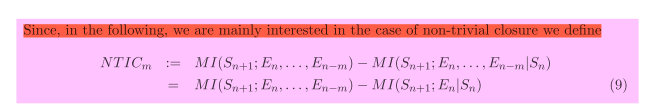
\includegraphics{WritingMaterials/PDFXCview_2018-06-01_17-44-30.png}
				
				@ or use 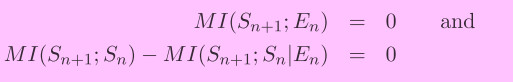
\includegraphics{WritingMaterials/PDFXCview_2018-06-04_19-18-12.png}
				
				@ To have high level non-trivial informational closure, the states of the coarse-grained scale need to
				
				@ First, maximise the mutual information between environment and the representation.
				This term implies that the agent need to maximise predictive power of environmental state. This also suggest that the environmental complexity is a crucial factor to the level of consciousness. The more rich and complex environment the agent try to predict the higher level of consciousness the agent has. 
				
				
				@ Second, to minimise the mutual information between environment and the representation conditional on the past state of the representation. This term suggests that the representation is self-predicable and it mimics the environmental transition. 
				
				@ Therefore, this theory predicts that level of consciousness determined by the environment that the agent adapts to. To form a high non-trivial informational closure, the agent will need to live in a complex environment and model the environmental transition precisely. 
				
				@ \rewording{Note that, our claim is that informational closure is a more fundamental property that correlates consciousness. A species acquiring advantage to model a complex environment through evolution and , therefore, achieving a high-level non-trivial informational closure has a high level of consciousness, is the consequence of the evolutional process. }
				
				
			\end{ants}
		
		
		
		\subsection{Conscious contents}
			\begin{ants}
				@ We claim that conscious contents correspond to the state of the informational closure. 
				
				@ \idea{= not sure I want to say this here =}
				
				@ Consciousness is informative. A conscious percept including volition and intention is a unique state that narrowing down all possible states into one. Therefore, a conscious percept reduces a huge amount of uncertainty. 
				
				@ This is the same claim as the third axiom called "information" in IIT. \needref{information axiom and need to say more about this.}
				
				@ ====================================
				
				@ Note that because the closure is at a coarse-grained scale one state of the informational closure can be mapped to several states at microscopic scale. 
			\end{ants}
		
		
		
		
		\subsection{Sensory hierarchy and neural coarse-graining
			\todo[color=Red]{This is super important. I need to deal with this very carefully. Need to completely rewording}}
		
			

			\begin{figure}[H]
				\includegraphicsTodo[width=0.8\textwidth]{hierarchy.pdf}
				\caption{Coarse-grain and sensory anatomical hierarchies}
				\label{fig:hierarchy}
			\end{figure}
		
			
			\begin{figure}[H]
				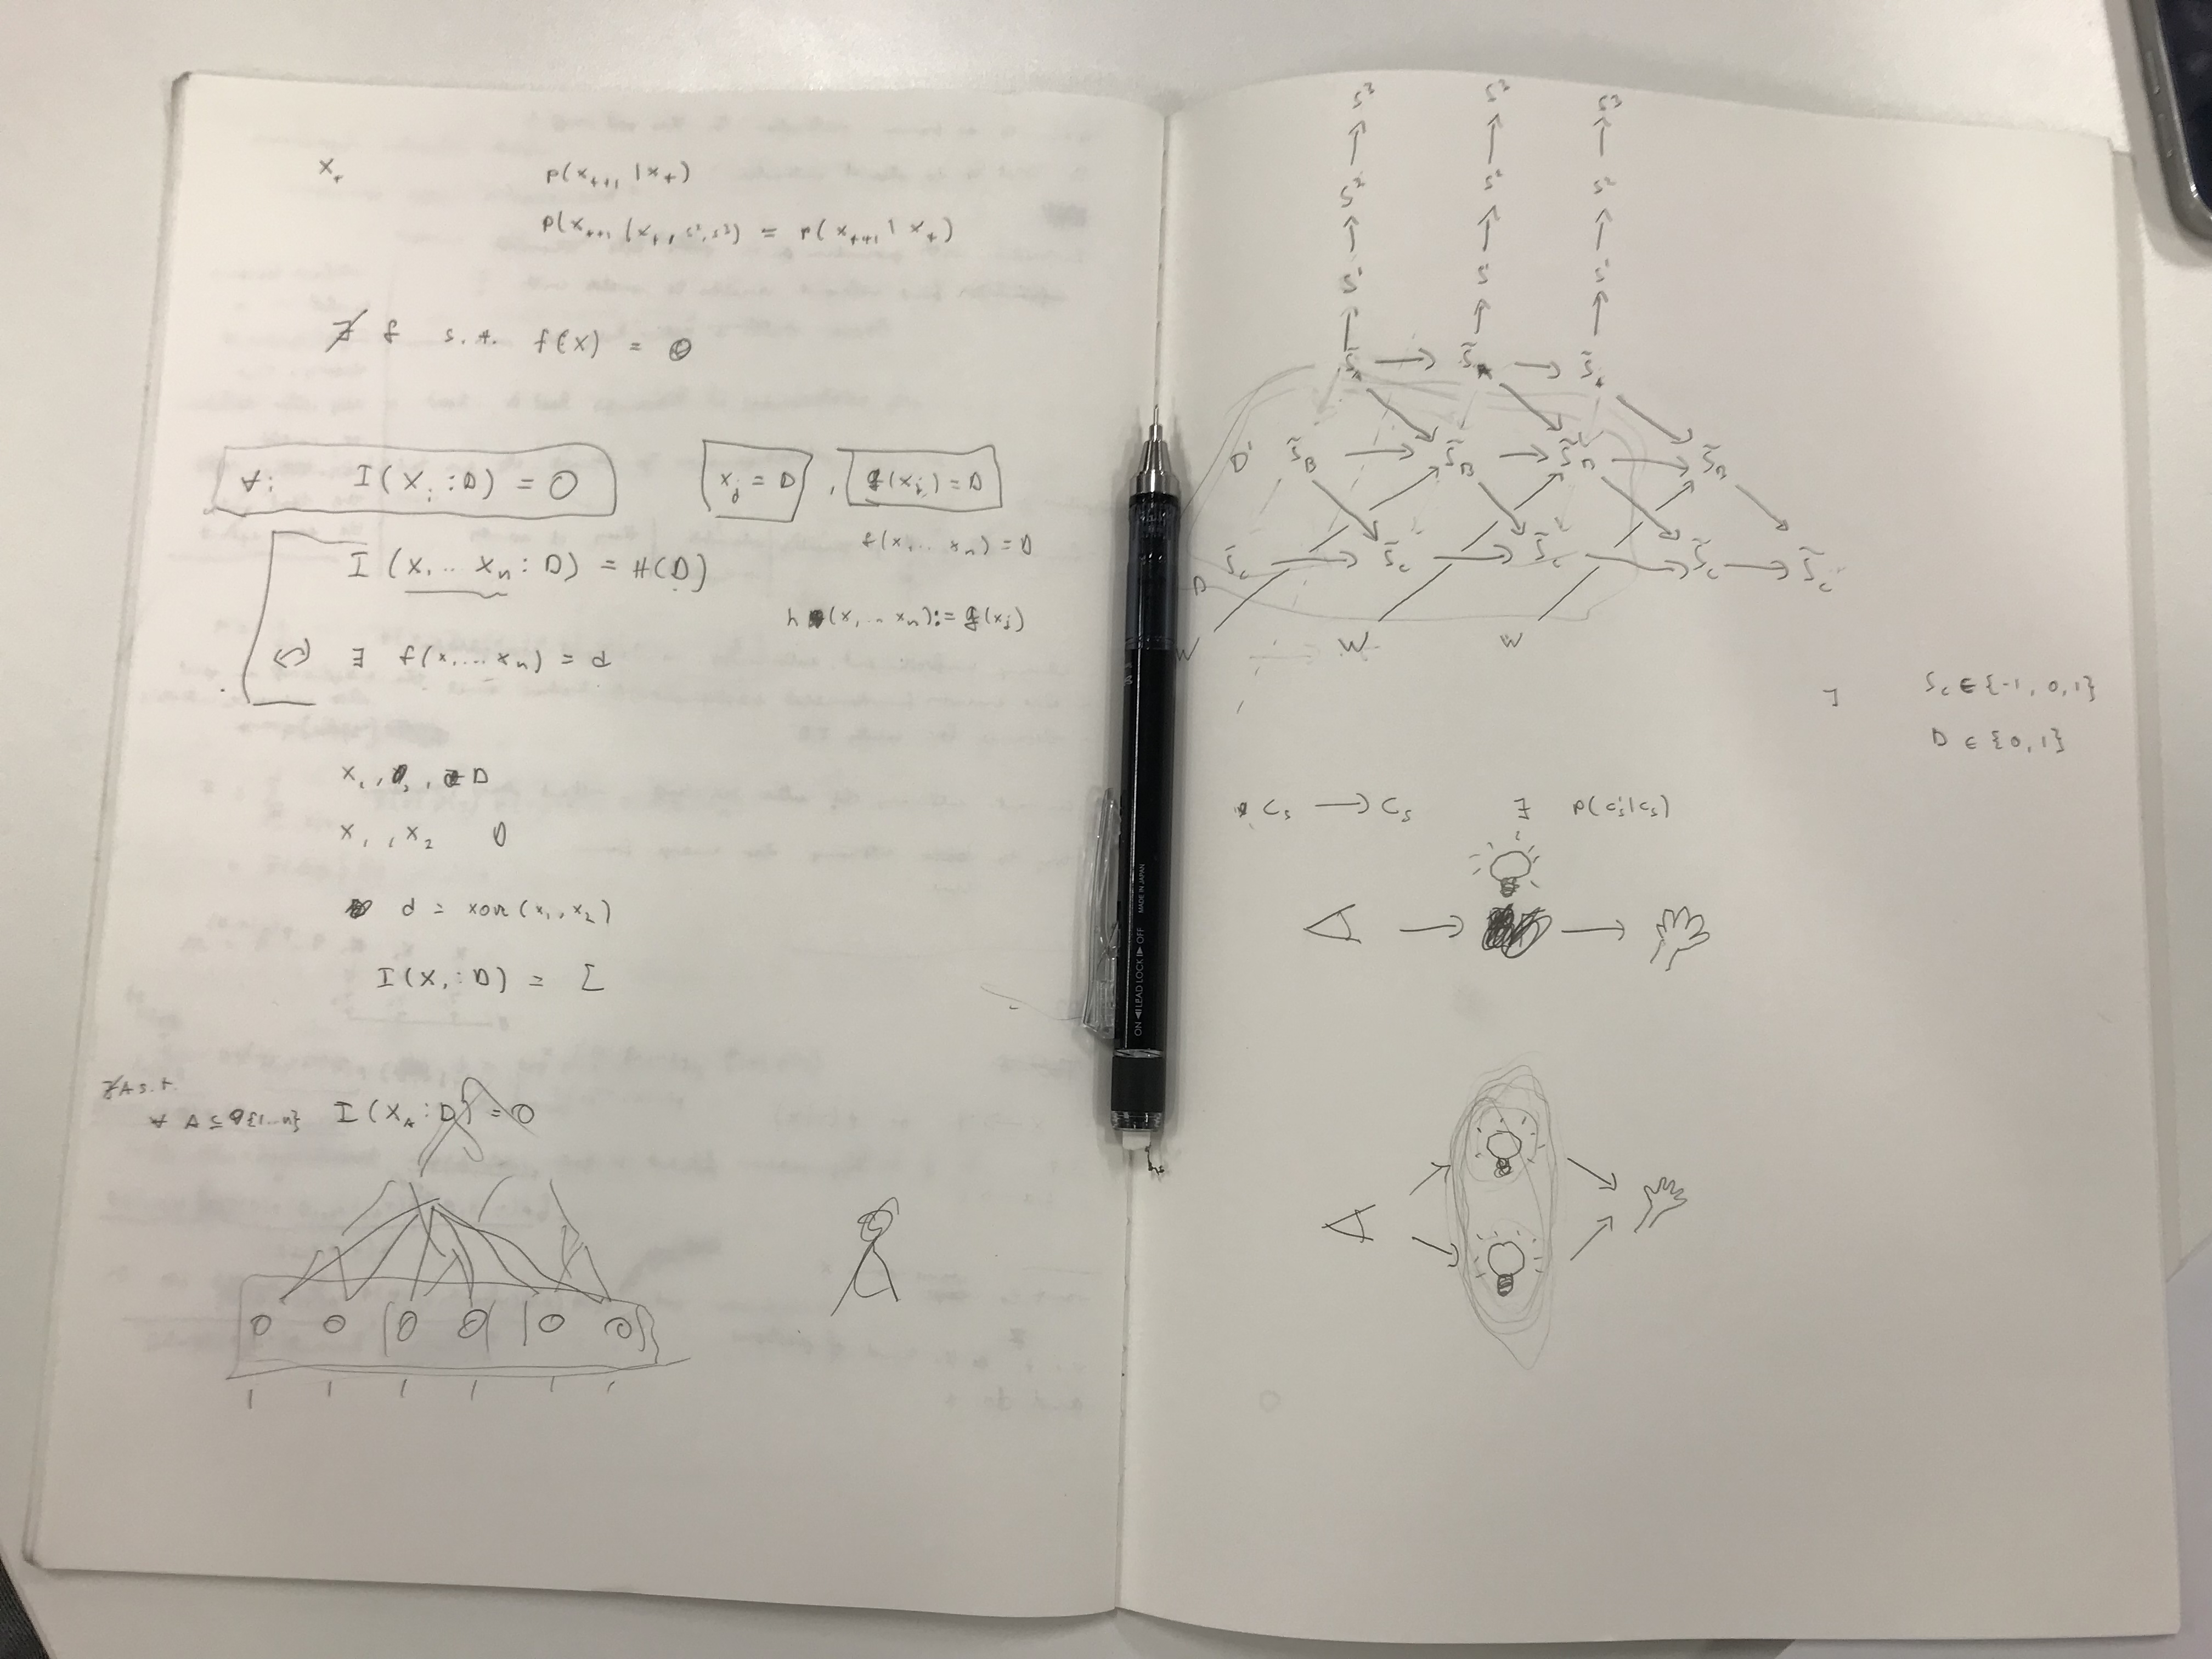
\includegraphics[width=\textwidth]{WritingMaterials/HierachyDiscussion (1).jpg}
%				{Coarse-grain and sensory anatomical hierarchies}
			\end{figure}		

		
		
		
			\begin{ants}
				@ It's important to note that the coarse-graining direction is not necessary to be align with anatomical sensory hierarchy in the neural system. 
				
				@ the coarse-grained information is needed and computed only when the information is required for microscopic scale processing. 
				
				@ \toWrite{I need a strong example here}
				
				
				@ Of course, from evolutional perspective, neural system should develop a better hardware to support neural coarse-graining
				
				@ For example, pooling layers in CNN is an implementation of coarse-graining function. It' is very plausible visual processing hierarchy in the neural system realises pooling layers. 
								
				
				@ It is possible that the neural system represents higher-level information processing by low level physical subtract. For example, studies have found representation for summery statistics of signal and neural. population.\needref{neural representation for summery statistics}\\
				From this point of view, sensory hierarchy may extend along with levels of coarse-graining.
				
				
				
			\end{ants}


		% ============================================================================ %
		%                         Information and system theory                        %
		%                                                                              %
		% ============================================================================ %
		\subsection{Information and system theory}
			\idea{A closure can define a system, consciousness is information}
			
			\idea{Could be linked to system theory, but may need help}
		
			\rewrite{
				This self-referential distinction from its environment therefore gives rise to the specific autonomy of such a system. Consequently, in systems theory, closure properties and autonomy are considered to be closely related concepts which are both at the heart of defining the system itself.}
			
			
			
		\subsection{Empirical approaches of measuring neural informational closure}
		
		
	\section{Biological evidence of informational closure in neural system}
		
		\begin{ants}		
			% ============================================================================ %
			%                             sederberg2018learning                            %
			% ============================================================================ %
			
			
			@ So far, not so much research on non-trivial informational closure in biological neural systems. 
			
			@ However, \rewording{XXX}
			
			% Internal self-predictive mechanism	
			@ Recent biological evidence suggests that low-level neurons encodes predictive information about external  and 
			
			@ \toWrite{
				need to say this is exactly the non-trivial informational closure, and refer to equation XXX}
			
			@ \cite{sederberg2018learning}
			@ \rewrite{
				in recordings of populations of RGCs of salamander retina driven by a simple stimulus with partially predictable dynamics, joint activity patterns transmit information that is predictive of future stimuli }
			
			@ \rewrite{
				We examined whether the temporal correlations within populations of RGCs can be used to guide the search for readouts of predictive information.}
			
			@ \rewrite{
				We showed that groups of cells with high external, stimulus-predictive information also had high internal predictive information on two classes of stimuli, }
			
			@ \rewrite{
				Very simple learning rules could find near-optimal readouts of predictive information without any external instructive signal. This suggests that bottom-up prediction may play an important role in sensory processing}
			
			@ \rewrite{
				Internal predictive information can guide stimulus prediction without explicit reference to stimulus parameters.}
			
			@ \rewrite{
				Word–word internal predictive information is correlated with word–stimulus predictive information across sets of four cells.}
			
			@ They also showed generalization of internal predictability across stimulus. This suggests .... what?
			
			@ \rewrite{
				The generalization of internal predictability across stimulus classes partially reflects the ability of the retina to adapt to the statistics of stimuli}
			
			
			@ \cite{Palmer2015}
			@ \rewrite{
				Groups of cells in the retina carry information about the future state of their own activity, and we show that this information can be compressed further and encoded by downstream predictor neurons that exhibit feature selectivity that would support predictive computations.}
			
			@ \rewrite{
				It seems natural to phrase the problem of prediction in relation to the visual stimulus, as in Fig. 3, but the brain has no direct access to visual stimuli except that provided by the retina. Could the brain learn, in an unsupervised fashion, to predict the future of retinal outputs? More precisely, if we observe that a population of retinal ganglion cells generates the word w t at time t, what can we say about the word that will be generated at time t + Δ t in the future? The answer to this question is contained in the conditional distribution of one word on the other, P ð w t +Δ t j w t Þ } \url{http://tinyurl.com/y9zmhlln}	
			
			@ \rewrite{
				larger groups of cells carry predictive information for hundreds of milliseconds, }
		
		\end{ants}




	\section{Relation to empirical findings in neuroscience and consciousness studies}
	
		\subsection{Unconscious Processing}
			\begin{ants}
				@ According the theory, there are two factor that renders neural processes unconscious. 
				
				@ First, processes are reflexive. This causes non-closured
				
				@ Second, the abstraction level of the information is below the non-trivial informational closure scale. 
			\end{ants}
		
		
	
		\subsection{reflexive behavioural is unconscious / or environment-state dependent}	
			\subsubsection{Reflection}
				\begin{ants}
					@ Reflexive systems is not informational closured. 
					@ Based on our theory, 
					@ x -> s -> a
						@@ the system state is determined by environmental state, then it is not conscious. 
					@ Therefore, in general, a simple policy network is not conscious. 
				\end{ants}
		
			\subsubsection{Blindsight}
				\begin{ants}
					@ This also blindsight. 
					@ Blindsight patients and still make above chance judgement without conscious awareness of visual targets.
					@ The stimulus-reaction policy network still intact, but it cannot form informational closure and therefore, patients has no conscious awareness of visual  targets
					@ Patient B.F. reactions are stimulus driven. 
				\end{ants}
		
			\subsubsection{procedure memory}
			
			\subsubsection{cerebellum}
				\begin{ants}
					@ cerebellum feed-forward connections, maybe just a policy network.\needref{cerebellum} 
				\end{ants}
				
		\subsection{Due to level of abstraction}
			\subsubsection{statistical inference}
				\begin{ants}
					@ The computation of Bayesian brain is unconscious.			 
				\end{ants}
			
			\subsubsection{subliminal perception}
			
			\subsubsection{Libet Experiments}		
		
			
		\subsection{Deterministic vs probabilistic}
			\cite{dehaene2017consciousness}
			\cite{vul2008temporal, moreno2011bayesian, asplund2014attentional, vul2009attention}
			
			
	\section{Phenomenology (conscious processing)}
	
			
		Binocular rivalry
		Hallucinations
		Dream / non-dream sleep
		planning 
		imagination 
	
		\subsection{Perceptual overflow}
		
	\section{Comparison with other theories}
		\subsection{Intermediate Level Theory}
		
			\begin{ants}
				@ \rewrite{
					The intermediate level theory originally proposed by Ray Jackendoff and further defended and specified by Jesse Prinz proposes that within the hierarchy of representations that are used to describe the cognitive system, conscious experience occurs only for specific levels of representation. The theory is rooted in Jackendoff ’s analysis of different cognitive systems such as vision, language, and music and the subsequent observation that consciousness does not arise anywhere within these systems. According to Jackendoff, consciousness is not associated with low-level, nor with high-level representations, but rather with those implying intermediate levels of processing. For instance, in the domain of object recognition, it is assumed that the visual system comprises a low level with local computations of visual features, an intermediate level reflecting binding and object recognition, and a higher level computing viewpoint invariance and representing abstract categories. According to Jackendoff and Prinz, conscious experience is not comprised of a disunified picture of visual features, nor is it represented by viewinvariant categories. Rather it is composed of bound and specific instances of objects that are assumed to be computed at the intermediate level of representation. In an analogous manner, speech perception can be decomposed into three levels: an acoustic representation of speech sounds at the lower level, a high level involving abstract lexical and syntactic categories, and in between a word recognition level relying on phonological representations. This theory explains why the conscious experience associated with speech perception mostly involves phonological representations, rather than other levels of representations. In Jackendoff and Prinz’ theory,the privileged role of the intermediate level of processing is based on the need for real-time computational efficiency. Indeed, this level of representation is assumed to be the most relevant one regarding ecological and functional needs. Another important aspect of this theory concerns the central role of attention during conscious experience. Here, attention is defined as a selection process that acts as a gate to working memory mechanisms. It performs the function of selecting the relevant information that is amplified afterward and then becomes conscious. Indeed, Prinz acknowledges that activation of an intermediatelevel representation on its own cannot be a sufficient condition for consciousness, given that those representations can be activated during subliminal perception. However, this theory makes the crucial postulate that the amplification of intermediatelevel representations by attention is a necessary and sufficient condition for consciousness. In sum, for each domain of processing, the content of consciousness at a particular moment is supported by a representational structure of intermediate level for that domain, which is selected to enter short-term memory, and enriched by attentional processing.} \cite{banks2009encyclopedia}
				
				@ \rewrite{
					In 1987, Ray Jackendoff published Consciousness and the Computational Mind. In it, he posed an important Where question: Where, in the fl ow of information, does consciousness arise? Most cognitive scientists agree that the mind is, in some sense, a computer. It is a device that processes information by transforming representations in accordance with rules. Computational devices decompose into various interconnected subsystems, each of which performs some aspect of a complex task. Given such a decompositional analysis, we can ask: in which subsystems does consciousness arise? If we depict the mind as a vast fl ow chart, and highlight the boxes whose rules and representations are conscious, which boxes should we mark? Jackendoff ’s answer is simple and elegant. He noticed that many of our mental capacities, including our senses and our language systems, are organized hierarchically. In each of these hierarchies, it makes sense to talk about low- , intermediate- , and high- level processing systems. We break down tasks into stages. Appealing to prevailing models of these stages, Jackendoff observed that the intermediate level seems to be privileged with respect to consciousness. Consciousness seems to arise in intermediate- level processing systems and not elsewhere.} \cite{prinz2007intermediate}
				
				@ \cite{jackendoff1987consciousness}
				@ \cite{prinz2007intermediate}
				@ 2.5D
			
			
				@ about why it is this level
				@@ \rewrite{
					Under the computational interpretation, the “why” question means: In what sense are intermediate level representations computationally important or distinctive? Th is is a tractable question, and it may lead to insights into the function of consciousness. Representations at the intermediate level are ideally suited for real- time deliberative behavioral responses. Low- level representations fail to bind features into coherent wholes. If we are going to interact with our environment, the low level is not a good guide. Th e high level is a good deal better for action, but also suboptimal. Th e high level tells us the category of the stimuli we perceive, but from an allocentric point of view. It abstracts away from stimulus features that are crucial for action. If we encounter a predator, the high- level visual representation does not tell us if it is facing toward us or away from us. Without that knowledge, we cannot decide what course of action to take. So, I propose that the intermediate level plays a distinctive role in information processing. It delivers representations that are coherent but viewpoint specifi c. Th ese representations are useful for determining what to do here and now.arg1} \cite{prinz2007intermediate}
				@@ \rewrite{
					I conclude that the intermediate level plays a distinctive and important computational role. Some researchers fi nd this puzzling. In wondering why the intermediate level is privileged, they note the arbitrariness of the fact that perceptual hierarchies have three levels. Could they not have two? Or a hundred? Do the 50 or so areas that contribute to visual processing really divide neatly into three levels? I think these puzzles depend on a particular understanding of what the word “intermediate” amounts to. One might get caught up in the fact that the intermediate level is the second stage in a sequence. Call this the “serial understanding of the intermediate level.” Alternatively, one might think of the intermediate level semantically. On this reading, the intermediate level is one that is not abstract and categorical, but not piecemeal or disunifi ed. Th ese notions are all in need of some refi nement, but, as a fi rst approximation, the idea is that intermediate- level representations are neither too specifi c nor too general.}\cite{prinz2007intermediate}
			\end{ants}
		
		
			\subsubsection{The difference between ILT and our theory}
				Prinz suggested that \rewrite{as. Cells in V1 are not promising candidates, because they do not reliably respond in ways that are consistent with features that we experience consciously. } \cite{prinz2007intermediate}
				
				* Our prediction is, if information that is carried by v1 neurons are necessary to complete informational closure, the states of V1 neurons should also co-vary with conscious contents. 	
				
		\subsection{first-order theories}
			\begin{ants}
				@\cite{lau2011empirical}
					@@ \rewrite{
						ddThe first-order view maintains that conscious awareness is determined by early sensory activity alone, independently of higher-order representations. Thus the crucial difference between the first-order and higher-order views is that the latter but not the former predict that conscious awareness is determined at least in part by prefrontal and parietal activity.\\
						Therefore, in the group of first-order theorists we include here not only those commonly labeled as such in the philosophical literature [11] but also theorists, such as Ned Block [12,13], who hold that the phenomenal qualities of awareness depend on the biological substrate rather than merely the content of the first-order representations, as well as scientists who hold that visual awareness depends on activity in content-specific regions of the extrastriate cortex [24,25] or on feedback from these regions to the primary visual cortex [26].\\
						Most first-order theories explain the difference between awareness and unawareness by positing that the latter is associated with weak information [29] or with representations in alternative (e.g. subcortical) sensory pathways. Thus this view suggests that conscious and unconscious processing will have different functional consequences. Whereas some first-order theorists hold that some higher cognitive functions can be performed without conscious awareness [30–32], most first-order theorists take a difference in perceptual task performance (e.g. ‘hits’ vs ‘misses’ in a detection task) as evidence for a difference in conscious awareness [12,13,25,26,33]. In other words, they typically associate task performance with awareness.}
				
			\end{ants}
		
		
		\subsection{Global Workspace Theory (GWT)}
			\subsubsection{Global availability and Broadcasting}
			
			\subsubsection{Code translation}
				\begin{ants}
					@ neural coarse-graining can natually solve this problem. 
					@ coarse-graining between levels can be thought as code translation\todo{is this true?}
				\end{ants}
			
			
			\subsubsection{Stability}
				\begin{ants}
					@ the presence of contexts as stable coalitions shaping access to the workspace.
					
				\end{ants}
			
			
			\subsubsection{broadcasting}
			
			\subsubsection{Ignition}
				\toWrite{Explain ignite}

		
			\begin{ants}
				@ GWT is one of the current popular consciousness theories.
				
				@ \rewrite{AI system and corresponds to our first functional definition of consciousness: global availability} \cite{Dehaene2017}
				
				@ C1: Global availability of relevant information The need for integration and coordination \cite{Dehaene2017}
				
				@ Evidence for integration and broadcasting
				
				@ Stability as a feature of consciousness \rewrite{“ meta-stability ” seems to be necessary for the nervous system to integrate information from a variety of modules and then broadcast it back to them, achieving flexible cross-module routing.}
				
				@ \rewrite{integration of computational resources in a large-scale coordination and for the exchange of information among processors}
				
				@ \rewrite{Grounded on the distinction between conscious and unconscious processes, Bernard Baars’ global workspace theory is one of the most influential cognitive theories of consciousness. This theory relies on the metaphor of a theater. In this theater, unconscious specialized processors (equivalent to modules) are assumed to be the actors and the audience. While the audience represents the set of passive processors, actors represents active processors playing on the stage of the theater (i.e., the workspace). These actors are engaged in a competition for being seen by the audience: by broadcasting their information they actually compete for more broadcasting. Active processors with the highest coherent activity can form local coalitions that strengthen them in this competition process. The strongest coalition in this competition dominates the workspace, in a winner-take-all fashion, and corresponds to the content of consciousness. The workspace is equated by Baars to working-memory, in which only the most active content becomes conscious. Additionally, the dominant coalition benefits from global broadcasting, which allows it to recruit new processors from the audience in order to form a global coalition. Here, consciousness allows for the integration of computational resources in a large-scale coordination and for the exchange of information among processors that would otherwise remain separated. In this theory, each processor can operate in the conscious mode if it benefits from global broadcasting through the workspace, or it can operate in the unconscious mode when disconnected from the workspace. An important feature of the global workspace theory is the presence of contexts as stable coalitions shaping access to the workspace. Contexts are constituted of unconscious processors reflecting, in a hierarchical manner, our expectations, our beliefs, our goals, and ultimately our self. In particular, attention is implemented as a goal context in this theory. It is described as a mechanism that controls access to the workspace, acting as a filter and biasing the competition process toward a particular set of actors. At any given moment, the dominant coalition is under the spotlight of attention, and its informational content becomes the content of conscious experience. A crucial aspect of Baars’ theory is that it avoids the problem of the homunculus by reducing it to an audience of multiple unconscious processors. Here, there is no need for a hypothetical single conscious observer in the system, and thus there is no issue of infinite regression with a homunculus inside another homunculus. Instead, consciousness is considered to reflect the global broadcasting of information to an audience of unconscious processors. As the audience is unconscious, unsupervised, and receptive rather than attending to the information, it does not constitute an internal homunculus.}
				
				
				
			\end{ants}
		
		
		

				
			
		\subsection{Higher Order Thought theory of consciousness}	
			\idea{
				People think a high order representation receives information from the first order representation. This may be a misunderstanding. This may be the result of neural coarse-graining. Because contents in informational closure look like watching fine-grained information, people may have an wrong impression about it}
		
			============================================================================			
			\begin{ants}
				@ Information closure directly is critical for other systems to construct forward models. 
				
				@ Therefore, most of the high level cognitions can utilise the state of informational closure.
				
				@ For example, mental planning needs a precise forward model to infer the environmental dynamics. 
				
				@ \idea{This is way HOT always involve consciousness }
				
				@ \cite{rosenthal2005consciousness}
			\end{ants}
		
		
			\rewrite{
				Higher-order theories of consciousness argue that conscious awareness crucially depends on higher-order mental representations that represent oneself as being in particular mental states.} \cite{lau2011empirical}
		
		
			\rewrite{
				According to this view, humans not only have first-order non-conceptual and/or analog perceptions of states of their environments and bodies, they also have second-order non-conceptual and/or analog perceptions of their first-order states of perception. And the most popular version of higher-order perception theory holds, in addition, that humans (and perhaps other animals) not only have sense-organs that scan the environment/body to produce fine-grained representations that can then serve to ground thoughts and action-planning, but they also have inner senses, charged with scanning the outputs of the first-order senses (i.e. perceptual experiences) to produce equally fine-grained, but higher-order, representations of those outputs (i.e. to produce higher-order experiences). A version of this view was first proposed by the British Empiricist philosopher John Locke (1690). In our own time it has been defended especially by Armstrong (1968, 1984) and by Lycan (1996).} \url{https://plato.stanford.edu/entries/consciousness-higher/#SelRepHigOrdThe}
			
			\rewrite{
				neutral about whether conscious awareness adds significant utility or immediate impact on behavior and task performance [1,27]. This is because the view assumes that task performance in most perceptual and cognitive tasks depends mainly on first-order rather than higher-order representations. Because conscious awareness can differ even if all first-order representations remain completely unchanged, such awareness itself might serve little function [1,27].}\cite{lau2011empirical} 		
				\ideaCallout{
					My theory would have similar prediction. Because conscious contents are coarse-grained results from low-level information. It is possible that more than two low-level neural states all coarse-grained to a high-level state.  }
					
			\subsubsection{Metacognition}
				\rewrite{
					Metacognition: cognition that is about another cognitive process as opposed to about objects in the world. In this article we use it mainly to refer to sensory metacognition: a cognitive process that concerns the quality or efficacy of a perceptual process. The capacity of sensory metacognition is sometimes empirically assessed by the correspondence between subjective report and task performance: how closely are they associated with each other on a trial-by-trial basis}\cite{lau2011empirical}

		
		\subsection{Sensorimotor contingency}
		\subsection{Predictive Brain}
			
			* Because of this XXXX, the representation has the maximal \ac{ntic} also has the maximal predictive power of the external environment. \todo[inline]{I need math here!!}
			
			
			* Therefore, it's reasonably assume that if evolution wants to build predictive mechanisms, the mechanisms should be settled on the information at the \ac{cged} level.
			
			* More specifically, a forward model, which received state and action as input and compute transition and then output next states, should be build on the representation that forms the \acl{ic}. 
			
			* Therefore, the state of predictive model can be conscious while it is linked to \acl{ic} representation. 
			
			* Note that, a system showing some predictive power is not sufficient to be conscious. 
			
			* For example, the proportional–integral–derivative controller (PID) controller shows predictive behaviours due to its derivative which computes and predict error value in the future. Derivative action predicts system behaviour and thus improves settling time and stability of the system. 
			
			* However, the state of the whole PID system still be determined by the inputs, i.e. the states of the controlled process, thus cannot complete \acl{ic}.
			
			. It can compute position, velocity, and acceleration of objects, and output control signals (action). However, the state of the PID controller is not information-closed. The state still fully determined by the input signals. Therefore, it fails to reach \ac{ic}. Hence, according to our theory, the PID system is not conscious. 
			
			* Similarly, the neural system also has many circuits that show predictive power but do not have \ac{ic}.
			
			
			\subsubsection{statistical learning/prediction is not conscious}
				\begin{ants}
					@ considers the brain as a predictive machine
					@ According to predictive processing account, conscious contents are the inference results (posterior from Bayesian inference framework) of predictive mechanism. 
					
					@ However, we can see that not all predictive mechanisms in the neural system can be consciously aware of. 
					
					@ So what's the critical difference between them in terms of consciousness?
					
					@ We argue that when predictive mechanisms utilise the information in the informational closure, the predictive result is conscious. 
					
					@ Because the forward model build on the informational closure representation can be seen as part of the closure. \todo[color=red]{IS THIS TRUE? NEED DISCUSSION}
					
					
					@ we can consider two scenarios
						
						@@ Predictive information is encoded in neuron populations but there is high entropy of conditional probability which means it's not closure. Therefore, the conscious level could be very low even though the it still has some degree of predictability. 
						
						@@ Another scenario is a forward model but its state fully depends on external sensory input. This system is not informational closured and therefore is not conscious. 
						
						@@ Based on this point of view, predictive power for a system does not guarantee consciousness. 
						
						@@ For example, in active inference \needref{active inference}, action is guided by prediction error so the state of the system is non-closured. 
					
				\end{ants}
				
			
		\subsection{Integrated information theory\callforhelp{Help from Jun?}}
			\begin{ants}
				@ \toWrite{Information integration without awareness}\cite{Mudrik_Faivre_Koch}
				@ \rewrite{consciousness is necessary for high-level but not low-level semantic integration}\cite{Mudrik_Faivre_Koch} I would argue an inverse relationship:"High-level information processing is necessary for consciousness." This is because higher-level information processing is more likely to create an informational closure representation. 
				
				@ Similarly, it is not \rewrite{consciousness is necessary for multisensory integration}. It should be multisensory integration is more likely to create an informational closure representation. Because in most situations, multisensory signals are generated from hidden causes which may have deterministic dynamic and relation with each other. Therefore, to infer the hidden causes and represent the deterministic relations can form informational closure representation which is conscious.  
				
			\end{ants}
						
			
			\subsubsection{Hoel's theory\callforhelp{Help from Marting?}}
				\ideaBox{This is very important. Need to be careful here.}
				
				
				\begin{ants}
					@ \cite{hoel2016can}
					@ causal emergence
					@ \cite{hoel2013quantifying} examined causal power at different coarse-grained scale and show that causal power can be stronger at macro rather than micro levels. 
					
					
					@ To answer the question about what is the best scale to compute Phi, \cite{hoel2016can} examined causal power at different coarse-grained scale. 
					
					@ Further instigation is needed to elucidate the relationship between our theory and causal emergence
					
					
				\end{ants}
				
				
		\subsection{Internal simulation and self-modelling}
		
		
		
	\section{Counter-intuitive prediction}	
	
		\subsection{informational closure}
			\begin{ants}
				@ We predict that through coarse-graining, conscious agents create 
			\end{ants}
			
			
		
		\subsection{Prediction on split-brain (vs IIT)}
			* IIT suggests that cutting, two subparts may both still have MIP, therefore, have two conscious mind. 
			
			* However, our theory suggests that if the cut largely destroy the \ac{ic}, then both part may not be conscious. 
	
	
	

	
	
	
	\section{Future works}
		\begin{ants}
			
			@ Lack of direct evidence because no one focus on informational closure
			
			@
			
		\end{ants}
	
		\subsection{Brain area}
		\subsection{attention}
		\subsection{How to coarse-grain in the neural system}
			\begin{ants}
				@ It's not clear what the coarse-graining function is.\todo[color=red]{this should be explained by environmental deterministic}
				
				@ \rewrite{
					not all causal relationships (or relationships of nomological dependency) among micro-events aggregate up to causal relationships among coarse-grained macro-events that are constituted by those micro-events. Instead, whether one gets causation at the macroscopic level will depend (among other things) on the particular coarse-graining that is chosen.} \cite{price2007causation}
				
				@ \rewrite{
					It may seem surprising, even counterintuitive, that causal and statistical dependence relationships involving fine grained microscopic variables do not automatically show up in causal and dependence relationships among the macroscopic variables that are realized by the fine grained variables.} \cite{price2007causation}
				
				@ \cite{jonas2017could} well demonstrated that it is difficult to understand higher-level information processing by the current neuroscience methods. 
				
			\end{ants}
	
	\section{Evolution of conscious mind (not sure but if I have time)}
		\cite{dennett2008kinds}
		

	\section{Conclusion}
		\begin{ants}
			@ Why is this theory better than other theories of consciousness
			@ NCC: To find NCC, it's not about where and when, it's about scale and level of description			 
		\end{ants}

	
	
	% ============================================================================ %
	%                                      End                                     %
	% ============================================================================ %
	
	\section*{Funding}
	
	\section*{Acknowledgements}
	
	\section*{Supplemental Data}
	
	\bibliographystyle{authordate1}
	\bibliography{ref}
	
	
	
\end{document}
